\chapter{Metodologia}

Para estudar a influência do sono na formação e recordação de conjuntos celulares será simulado
um modelo de RND com diferentes formas de plasticidade. A rede será composta de 
5120 neurônios IF, sendo 4096 excitatórios e 1024 inibitórios.


criar a RND
vai ter x neurônios, y excitatórios...

estímulos
vão ser tais estímulos, a rede vai ter uma retina, nenhum estímulo significa X aleatório...

modelo de neurônio
vai ser o modelo IF de tal jeito

modelo de plasticidade
vão ser implementados tais tipos de plasticidade seguindo as seguintes regras

simulação do sono
o sono vai ser ativado e desativado dependendo no tempo
durante o sono, a retina não vai ver nada
o sono vai ter fases
dependendo da fase, vai ser injetada corrente sinoidal nos neurônios de forma a imitar os padrões do sono




\section{Cronograma}

\begin{table}[!ht]
\Caption{Cronograma de atividades.}
\centering\label{fig_cronograma}
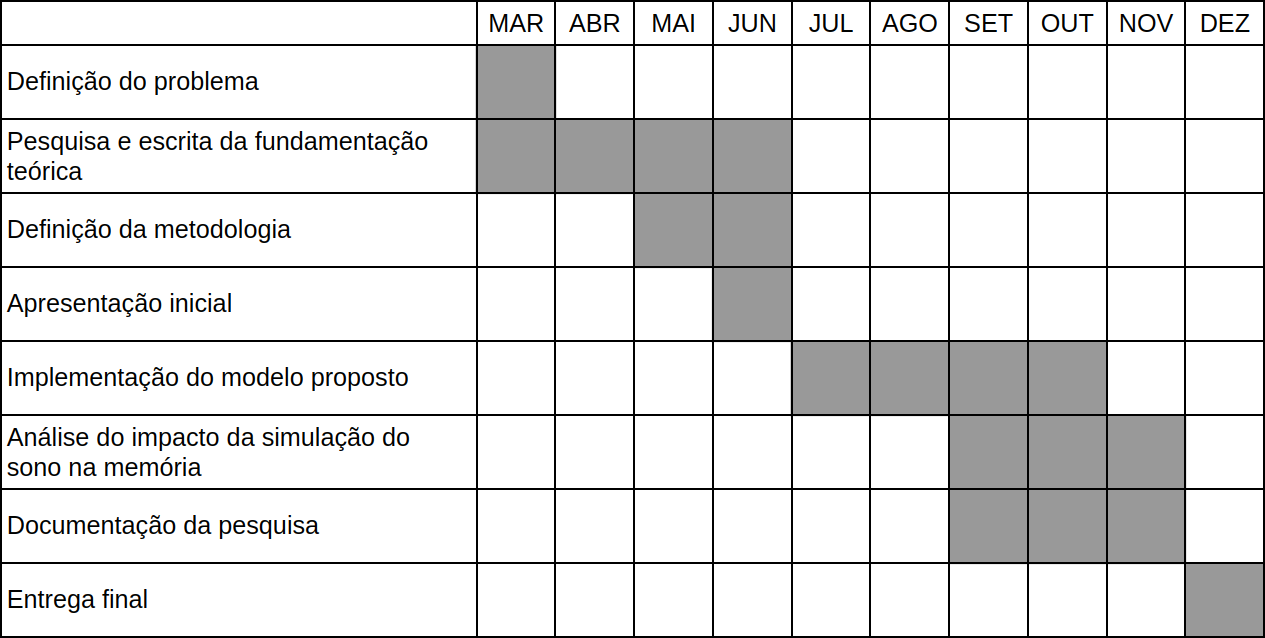
\includegraphics[width=\linewidth]{figuras/cronograma.png}
% \Fonte{}
\end{table}